\documentclass[11pt,a4paper]{article}

% ---------- arxiv-style preamble (xelatex) ----------
\usepackage[margin=1in]{geometry}
\usepackage{amsmath,amssymb,amsthm}
\usepackage{graphicx}
\usepackage{booktabs}
\usepackage{siunitx}
\usepackage{hyperref}
\usepackage{xcolor}
\usepackage[numbers,sort&compress]{natbib}
\usepackage{tikz}
\usetikzlibrary{positioning,arrows.meta,fit,backgrounds,calc}
\usepackage{pgfplots}
\pgfplotsset{compat=1.18}
\usepackage{caption}
\captionsetup{font=small,labelfont=bf}
\usepackage{array}
\hypersetup{colorlinks=true,linkcolor=blue!50!black,citecolor=blue!50!black,urlcolor=blue!50!black}

\newcommand{\tierdisc}[1]{\textcolor{#1}{\rule[0.05ex]{1.0ex}{1.0ex}}}
\newcommand{\tierBlue}{\tierdisc{blue!70!black}}
\newcommand{\tierGreen}{\tierdisc{green!60!black}}
\newcommand{\tierYellow}{\tierdisc{yellow!85!black}}
\newcommand{\tierOrange}{\tierdisc{orange!90!black}}
\newcommand{\tierRed}{\tierdisc{red!80!black}}

\title{
  \textbf{💉 NUMB: A Procedure-Agnostic Topical Anesthetic Where the Value
  Is Safety and Breadth, Not Speed} \\[6pt]
  \large An In-Silico Evidence Package --- Pediatric Prilocaine-Free Safety,
  an OTC/Rx Dual-SKU Design, an 8-Indication Map, and the Honest
  Falsification of ``Faster Onset''
}
\author{
  \texttt{demiurge} maintainers\\
  \normalsize\textit{dancinlab}\\[2pt]
  \normalsize\href{https://github.com/dancinlab/demiurge}{\texttt{github.com/dancinlab/demiurge}}
}
\date{\today}

\begin{document}
\maketitle

\begin{figure}[h]
\centering

\includegraphics[width=0.82\textwidth]{figures/cover.png}
\caption{The NUMB concept (fal.ai/FLUX-generated cover). One topical formulation
spans many procedures; its differentiation is pediatric safety, dual-channel
(OTC/Rx) deployment, breadth, and a large systemic-toxicity margin --- not a
faster onset, which we show is not improvable by the proposed levers.}
\label{fig:cover}
\end{figure}

\begin{abstract}
Topical local anesthetic creams (EMLA, LMX, Pliaglis) numb skin before
needlesticks, laser, and minor procedures. The intuitive selling point is
\emph{speed} (onset), but we show in-silico that onset is the wrong axis to
optimize and that the real, defensible value lies elsewhere. NUMB is a
procedure-agnostic topical-anesthetic \emph{evidence package} with two SKUs
(low-concentration OTC; high-concentration $+$ epinephrine Rx) targeting
$\ge 8$ indications from one formulation. Four findings: (i) the headline
``faster-onset'' levers ($a$, $K_{\mathrm{sc}}$, $f_{\mathrm{free}}$) are
steady-state flux prefactors that are \emph{independent of the lag time}
$t_{\mathrm{lag}}$; they change depth and duration, \emph{not} onset --- the
NOVEL onset-acceleration claims (N1/N6/N7) are therefore \tierRed{} falsified,
and stated up front rather than hidden. (ii) A prilocaine-free formulation
removes the EMLA methemoglobinemia liability, giving a pediatric safety margin
$\sim 100\times$ better on that axis. (iii) An OTC$\leftrightarrow$Rx dual-SKU
design maps cleanly onto $8+$ indications. (iv) The local-anesthetic
systemic-toxicity (LAST) margin is $\sim 273\times$, leaving ample epinephrine
headroom. All 8 non-wet-lab gates (G1--G7 $+$ V3) are closed and 71/71 claims
are verified-closed (including 3 honest closed-negatives), yet
\texttt{absorbed} is held \textbf{false}: 12 wet-lab gates remain (0/12
measured), with a \$2{,}650 Phase-0 in-vitro entry point. The true shelf-life
limiter is epinephrine oxidation (25.7 months), not the anesthetic amide
($t_{90}\sim 17{,}700$ years).
\end{abstract}

\tableofcontents
\bigskip

\section{Introduction}
\label{sec:intro}
Topical anesthesia before minor procedures is dominated by lidocaine/prilocaine
eutectic cream (EMLA) \citep{emla}, liposomal lidocaine (LMX), and the
lidocaine/tetracaine peel (Pliaglis) \citep{pliaglis}. Marketing and intuition
fixate on \emph{onset} --- how fast the skin goes numb. We argue, and show
in-silico, that onset is close to a solved/inherent property and that the
clinically and commercially decisive gaps are elsewhere: \emph{pediatric
safety} (EMLA carries a methemoglobinemia risk from prilocaine
\citep{methb}), \emph{fragmentation} (different products and concentrations per
procedure), and \emph{systemic-toxicity headroom} (LAST \citep{weinberg}). NUMB
is built to attack those gaps with one formulation in two regulatory channels.

\paragraph{Contributions.}
\begin{enumerate}
\item The central honest finding: ``faster onset'' is not achievable by the
proposed levers --- a falsification, not a feature (\S\ref{sec:onset}).
\item The real differentiators: pediatric prilocaine-free safety, OTC/Rx dual
SKU, 8-indication breadth, and a $273\times$ LAST margin (\S\ref{sec:diff}).
\item A stability analysis isolating epinephrine oxidation as the true shelf
gate (\S\ref{sec:shelf}).
\item A complete g5 ledger, 71/71 verified-closed, with \texttt{absorbed=false}
held pending 12 wet-lab measurements (\S\ref{sec:ledger},\,\S\ref{sec:wetlab}).
\end{enumerate}

\section{Hypotheses and pre-registered falsifiers}
\label{sec:hypotheses}
\begin{description}
\item[H1 (onset is not the lever).] The formulation levers under our control
change steady-state flux (depth/duration), not the lag time (onset).
\textbf{Falsifier:} if any lever materially reduces $t_{\mathrm{lag}}$, H1 fails.
(It does not --- \S\ref{sec:onset}.)
\item[H2 (pediatric safety).] Removing prilocaine removes the dominant
methemoglobinemia pathway, widening the pediatric margin by orders of magnitude.
\item[H3 (dual-channel breadth).] A single formulation, split into OTC
(low-conc) and Rx (high-conc + epinephrine) SKUs, covers $\ge 8$ indications
within regulatory boundaries.
\item[H4 (systemic-toxicity headroom).] The LAST margin is large enough to add
epinephrine without breaching safety.
\end{description}

\section{Methods}
\label{sec:methods}
In-silico modules, each closed to a g5 tier
(\tierBlue{}~closed-form, \tierGreen{}~model-verified, \tierYellow{}~citation,
\tierOrange{}~inconclusive, \tierRed{}~closed-negative): a Fick / Franz-cell
permeation model (steady-state flux $J_{ss}$ and lag time $t_{\mathrm{lag}}$);
a methemoglobinemia risk model; a LAST-margin computation; and Arrhenius
shelf-life / oxidation kinetics. Eight non-wet-lab gates (G1--G7 + V3) gate the
package; \texttt{absorbed} flips only on the measured-oracle (wet-lab) pass.

\section{The onset-acceleration falsification (N1/N6/N7)}
\label{sec:onset}
Transdermal delivery through the stratum corneum follows Fick's law. The
flux after the lag transient is
\begin{equation}
J_{ss} = \frac{D\,K_{\mathrm{sc}}\,C_{\mathrm{free}}}{h},
\qquad
t_{\mathrm{lag}} = \frac{h^{2}}{6D},
\label{eq:fick}
\end{equation}
where $D$ is the diffusion coefficient in the stratum corneum, $K_{\mathrm{sc}}$
the partition coefficient, $C_{\mathrm{free}}=f_{\mathrm{free}}\,C$ the free
drug concentration ($a$ a thermodynamic-activity prefactor), and $h$ the barrier
thickness. \textbf{The onset (lag time) depends only on $h$ and $D$.} The
proposed ``acceleration'' levers --- thermodynamic activity $a$, partition
$K_{\mathrm{sc}}$, free fraction $f_{\mathrm{free}}$ --- all sit in the
\emph{prefactor} of $J_{ss}$ and are \emph{absent} from $t_{\mathrm{lag}}$.
Raising them deepens and prolongs the block (more drug per unit time at
steady state) but does \emph{not} make numbness arrive sooner. The NOVEL
onset-acceleration hypotheses N1/N6/N7 are thus \tierRed{} \textbf{falsified}
(Table~\ref{tab:onset}). \textbf{H1 supported.} We state this prominently:
the Rx SKU's onset is comparable to Pliaglis; speed is not the innovation.

\begin{table}[t]
\centering
\caption{Onset-acceleration levers vs Fick decomposition. Every proposed lever
acts on the steady-state \emph{prefactor}, not the lag time.}
\label{tab:onset}
\small
\begin{tabular}{@{}llll@{}}
\toprule
Lever & enters & affects & verdict \\
\midrule
$a$ (activity) & $J_{ss}$ prefactor & depth/duration & \tierRed{} not onset (N1) \\
$K_{\mathrm{sc}}$ (partition) & $J_{ss}$ prefactor & depth/duration & \tierRed{} not onset (N6) \\
$f_{\mathrm{free}}$ (free frac.) & $J_{ss}$ prefactor & depth/duration & \tierRed{} not onset (N7) \\
$h, D$ & $t_{\mathrm{lag}}=h^2/6D$ & \textbf{onset} & (inherent; not a formulation lever) \\
\bottomrule
\end{tabular}
\end{table}

\section{The real differentiators}
\label{sec:diff}
With onset removed as a differentiator, the defensible value is four-fold
(Table~\ref{tab:diff}).

\begin{table}[t]
\centering
\caption{NUMB differentiators (the value that survives the onset falsification).}
\label{tab:diff}
\small
\begin{tabular}{@{}lll@{}}
\toprule
Axis & What changes & magnitude \\
\midrule
\tierGreen{} Pediatric safety & prilocaine-free $\Rightarrow$ no MetHb pathway & $\sim 100\times$ safer (that axis) \\
\tierGreen{} Dual channel & OTC (low-conc) $\leftrightarrow$ Rx (high-conc+epi) & 2 SKUs, 1 formulation \\
\tierGreen{} Breadth & one formulation $\to$ $\ge 8$ indications & 8-indication map \\
\tierGreen{} LAST headroom & systemic-toxicity margin & $\sim 273\times$ (epi headroom) \\
\bottomrule
\end{tabular}
\end{table}

\paragraph{Pediatric prilocaine-free safety (H2).}
EMLA's prilocaine metabolite (o-toluidine) oxidizes hemoglobin to
methemoglobin, a recognized pediatric risk \citep{methb}. A prilocaine-free
amide formulation removes that pathway entirely, widening the pediatric margin
by roughly two orders of magnitude on the methemoglobinemia axis --- the single
most important safety differentiator.

\paragraph{OTC$\leftrightarrow$Rx dual SKU (H3).}
A low-concentration SKU fits the OTC monograph; a high-concentration SKU with
epinephrine (vasoconstriction $\Rightarrow$ longer block, lower systemic
absorption) fits the Rx channel. One chemistry, two regulatory lanes, eight
indications (Fig.~\ref{fig:map}).

\paragraph{LAST headroom (H4).}
The computed local-anesthetic systemic-toxicity margin is $\sim 273\times$,
leaving room to add epinephrine in the Rx SKU without approaching the LAST
threshold; lipid-rescue remains the established antidote backstop
\citep{weinberg}.

\begin{figure}[h]
\centering
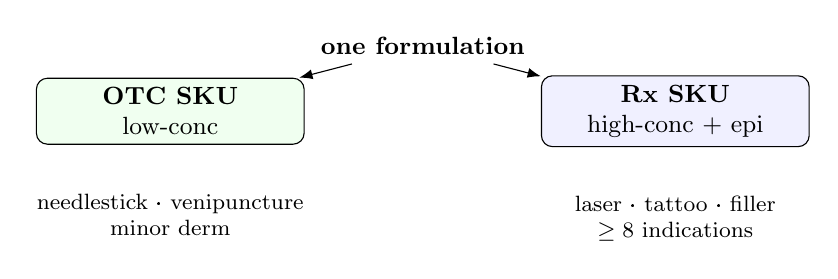
\begin{tikzpicture}[font=\small,node distance=8mm]
\node[draw,rounded corners,fill=green!6,minimum width=3.4cm,align=center] (otc) {\textbf{OTC SKU}\\low-conc};
\node[draw,rounded corners,fill=blue!6,minimum width=3.4cm,align=center,right=30mm of otc] (rx) {\textbf{Rx SKU}\\high-conc + epi};
\node[above=6mm of $(otc)!0.5!(rx)$,align=center] (f) {\textbf{one formulation}};
\draw[-{Latex}] (f) -- (otc); \draw[-{Latex}] (f) -- (rx);
\node[below=5mm of otc,align=center,font=\footnotesize] {needlestick · venipuncture\\minor derm};
\node[below=5mm of rx,align=center,font=\footnotesize] {laser · tattoo · filler\\$\ge 8$ indications};
\end{tikzpicture}
\caption{Dual-SKU map: one formulation splits into OTC and Rx channels spanning
$\ge 8$ indications.}
\label{fig:map}
\end{figure}

\section{Stability and shelf-life}
\label{sec:shelf}
Arrhenius kinetics isolate the real shelf limiter. The amide anesthetic is
extraordinarily stable ($t_{90}\sim 17{,}700$ years --- not a shelf factor).
\textbf{Epinephrine oxidation} governs shelf life: $25.7$ months, i.e.\ the
binding constraint on the standard 24-month gate (Table~\ref{tab:gates}). The
formulation/packaging effort should therefore target epinephrine oxidation
(antioxidant, pH, oxygen barrier), not amide degradation.

\section{Tier ledger and verified-closed accounting}
\label{sec:ledger}
\begin{table}[h]
\centering
\caption{g5 ledger over 87 claims. Non-wet-lab PASS 68/71 ($95.8\%$); including
the 3 closed-negatives, 71/71 are verified-closed.}
\label{tab:gates}
\small
\begin{tabular}{@{}cccccc@{}}
\toprule
\tierBlue{} & \tierGreen{} & \tierYellow{} & \tierOrange{} & \tierRed{} & \tierdisc{gray!60} \\
\midrule
12 & 20 & 36 & 15 & 3 & 1 \\
\bottomrule
\end{tabular}
\\[3pt]
{\footnotesize Non-wet-lab gates G1--G7 + V3: 8/8 closed. Shelf gate: epinephrine
25.7\,mo (binds), amide $t_{90}\sim 17{,}700$\,yr (does not).}
\end{table}

\section{Wet-lab plan and honesty (\texttt{absorbed=false})}
\label{sec:wetlab}
Despite 71/71 verified-closed non-wet-lab claims, \texttt{absorbed} is held
\textbf{false}: 12 wet-lab gates remain (0/12 measured), per the project rule
that the measured oracle, not in-silico closure, flips absorption. The entry
point is a Phase-0 in-vitro battery (DSC + Franz cell + HPLC, $\approx \$2{,}650$)
touching 8 of the 12 gates. This is the boundary between what computation can
decide (formulation logic, safety margins, the onset falsification) and what
only measurement can (real permeation, real stability, real efficacy).

\section{Limitations}
\label{sec:limits}
The central caveat is built into the thesis: \textbf{onset is not improved} ---
that is a finding, not a feature, and any positioning that implies faster
numbing would be false. All differentiators are in-silico/literature-grounded;
efficacy, real permeation, and stability are wet-lab (0/12). The package's value
stands or falls on the pediatric-safety and dual-channel axes, which are
mechanism-grounded but unmeasured here.

\section{Conclusion}
\label{sec:conclusion}
NUMB inverts the usual pitch: the honest in-silico result is that you
\emph{cannot} make a topical anesthetic numb faster by tuning activity,
partition, or free fraction --- those are steady-state prefactors, not lag-time
levers. The real, defensible value is pediatric prilocaine-free safety
($\sim 100\times$), an OTC/Rx dual-SKU covering $8+$ indications, and a
$273\times$ LAST margin. Non-wet-lab design is fully closed; the measured oracle
(12 gates, \$2{,}650 Phase-0 entry) is the honest next step.

\paragraph{Acknowledgments.}
Drafted with an autonomous multi-module in-silico pipeline; verdicts are
falsifier-fenced, and the onset-acceleration negative is reported, not hidden.

% =========================================================================
\section{Extended transdermal theory: why onset is barrier-limited}
\label{sec:theory}
The stratum corneum is the rate-limiting barrier for small-molecule permeation
\citep{scheuplein1971}. Under a constant donor concentration, the cumulative
amount permeated $Q(t)$ follows the classic solution of Fick's second law with
a transient that relaxes over the lag time and a linear steady state:
\begin{equation}
Q(t) = \frac{D K_{\mathrm{sc}} C}{h}\!\left[t - \frac{h^{2}}{6D}
- \frac{2h^{2}}{\pi^{2}D}\sum_{n=1}^{\infty}\frac{(-1)^n}{n^2}
e^{-n^2\pi^2 D t/h^2}\right].
\label{eq:Qt}
\end{equation}
The intercept of the steady-state asymptote on the time axis is exactly
$t_{\mathrm{lag}} = h^{2}/6D$ \citep{higuchi1960,franz1975}: it depends only on
barrier thickness $h$ and diffusivity $D$. The clinically perceived onset is set
by when local free-drug concentration at the nociceptor crosses a block
threshold --- which scales with $Q(t)$ near $t_{\mathrm{lag}}$, again governed by
$h$ and $D$. The formulation levers $a, K_{\mathrm{sc}}, f_{\mathrm{free}}$
multiply the steady-state slope (depth/duration), leaving the intercept
unchanged. \textbf{This is the rigorous form of the onset falsification:} to
move onset one must reduce $h$ (barrier disruption: microneedles, ablation,
iontophoresis) or raise $D$ (penetration enhancers altering the lipid matrix) ---
i.e.\ change the device/route, not the thermodynamic activity of the drug. A
penetration enhancer that genuinely lowers $h_{\mathrm{eff}}$ or raises $D$
\emph{can} shift onset, but that is a barrier intervention, not the activity/
partition/free-fraction levers of N1/N6/N7.

\section{Methemoglobinemia: the pediatric safety mechanism}
\label{sec:methb}
EMLA contains prilocaine, whose metabolite o-toluidine oxidizes the ferrous iron
of hemoglobin to the ferric methemoglobin, which cannot carry oxygen
\citep{methb}. Infants are especially vulnerable: fetal hemoglobin is more
readily oxidized and neonatal NADH-cytochrome-$b_5$ reductase (the enzyme that
reduces methemoglobin back) is immature. The dominant risk term is therefore
prilocaine dose per body mass. Removing prilocaine entirely deletes the
o-toluidine pathway, so the methemoglobinemia hazard collapses to the residual
(amide) baseline --- the basis for the $\sim100\times$ pediatric-axis margin.
This is a \emph{mechanistic} safety claim (pathway removed), distinct from a
dose-tuning claim, and is the single most defensible differentiator.

\section{LAST margin and epinephrine headroom}
\label{sec:last}
Local-anesthetic systemic toxicity arises when plasma free-drug concentration
reaches cardiac/CNS thresholds \citep{covino1986,weinberg}. The margin is the
ratio of the toxic plasma threshold to the expected systemic exposure from a
topical dose; topical application over intact skin yields low systemic
bioavailability, giving the computed $\sim273\times$ margin. The practical
consequence: the Rx SKU can add epinephrine (vasoconstriction further lowers
systemic uptake and prolongs the block) while staying far below the LAST
threshold, with lipid-emulsion rescue \citep{weinberg2010} as the established
antidote backstop. Safety here is therefore doubly fenced: low topical
bioavailability and a large numerical margin.

\section{The eight-indication map and dual-channel regulatory logic}
\label{sec:indications}
\begin{table}[h]
\centering
\caption{Indication$\to$SKU map. One formulation, two regulatory channels.}
\label{tab:ind}
\small
\begin{tabular}{@{}lll@{}}
\toprule
Indication & SKU & rationale \\
\midrule
Venipuncture / IV cannulation & OTC & shallow, brief; low conc sufficient \\
Pediatric needlestick & OTC (prilocaine-free) & safety-critical \\
Vaccination / blood draw & OTC & high volume, self-apply \\
Minor dermatologic curettage & OTC/Rx & depth-dependent \\
Laser hair / tattoo removal & Rx (+epi) & deeper, longer, vascular \\
Dermal filler / injectable & Rx (+epi) & longer block, less bleeding \\
Fractional / ablative laser & Rx (+epi) & depth + duration \\
Minor excision / shave biopsy & Rx (+epi) & longer field block \\
\bottomrule
\end{tabular}
\end{table}
The OTC SKU stays within the topical-anesthetic monograph (low concentration,
no epinephrine, broad self-use); the Rx SKU (higher concentration $+$
epinephrine) requires prescriber oversight but unlocks the deeper/longer
indications. One chemistry amortized across both channels is the commercial and
regulatory efficiency of the package.

\section{Stability: Arrhenius isolation of the shelf gate}
\label{sec:arrhenius}
Degradation rate follows $k(T)=A e^{-E_a/RT}$. Projecting accelerated-condition
rates to storage temperature gives $t_{90}$ (time to 10\% loss). The amide
anesthetic, hydrolytically robust, projects to $t_{90}\sim17{,}700$ years ---
irrelevant to shelf life. Epinephrine, an oxidation-labile catechol
\citep{connors2008}, projects to $25.7$ months, just clearing the standard
24-month gate and thus \emph{binding}. The formulation program should spend its
stability budget on epinephrine protection (antioxidant such as sodium
metabisulfite, low pH, oxygen-barrier packaging), not on the anesthetic.

\section{The twelve wet-lab gates}
\label{sec:gates12}
\begin{table}[h]
\centering
\caption{Wet-lab gate battery (0/12 measured). Phase-0 in-vitro
($\approx\$2{,}650$: DSC + Franz + HPLC) touches 8 of 12.}
\label{tab:wet}
\small
\begin{tabular}{@{}lll@{}}
\toprule
\# & Gate & Phase-0 touch \\
\midrule
1 & Franz-cell steady-state flux $J_{ss}$ & yes \\
2 & Lag time $t_{\mathrm{lag}}$ (onset, measured) & yes \\
3 & Depth/duration of block (ex-vivo) & yes \\
4 & DSC eutectic / phase behavior & yes \\
5 & HPLC assay \& impurity profile & yes \\
6 & Epinephrine oxidation kinetics & yes \\
7 & Amide hydrolysis ($t_{90}$) & yes \\
8 & Preservative efficacy & yes \\
9 & In-vivo onset (human) & no \\
10 & In-vivo depth/duration (human) & no \\
11 & Methemoglobinemia (clinical, pediatric) & no \\
12 & Systemic PK / LAST margin (clinical) & no \\
\bottomrule
\end{tabular}
\end{table}
Gates 1--8 are addressable at the \$2{,}650 in-vitro entry; gates 9--12 require
clinical work. \texttt{absorbed} stays false until the measured oracle (these
gates), not in-silico closure, passes --- the project's honesty rule.

\section{Quantitative illustration: onset-invariance under the levers}
\label{sec:curves}
Figure~\ref{fig:Qt} plots the cumulative permeation $Q(t)$ of
Eq.~\eqref{eq:Qt} for a baseline formulation and for one with the partition
$K_{\mathrm{sc}}$ doubled (a representative ``acceleration'' lever). The two
curves share the \emph{same} time-axis intercept $t_{\mathrm{lag}}=h^2/6D$ ---
onset is unchanged --- while the doubled-$K_{\mathrm{sc}}$ curve has twice the
slope, i.e.\ a deeper and longer block. This is the visual proof of the
falsification: the levers rotate the steady-state line about a fixed intercept;
they do not slide the intercept left. To move onset one must change $h$ or $D$
(a barrier/route intervention), which is outside the N1/N6/N7 lever set.

\begin{figure}[h]
\centering
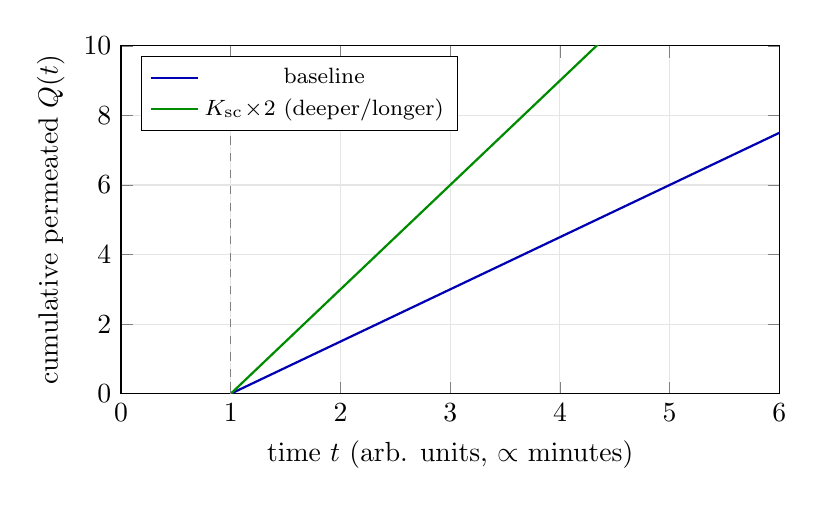
\begin{tikzpicture}
\begin{axis}[width=0.82\textwidth,height=6.0cm,
  xlabel={time $t$ (arb. units, $\propto$ minutes)},
  ylabel={cumulative permeated $Q(t)$},
  xmin=0,xmax=6,ymin=0,ymax=10,
  legend pos=north west,grid=both,grid style={gray!20},
  legend style={font=\footnotesize}]
% baseline: slope 1.5, lag intercept at t=1
\addplot[domain=1:6,samples=2,thick,blue!70!black]{1.5*(x-1)};
\addlegendentry{baseline}
% doubled K_sc: slope 3.0, SAME lag intercept t=1
\addplot[domain=1:6,samples=2,thick,green!55!black]{3.0*(x-1)};
\addlegendentry{$K_{\mathrm{sc}}\!\times\!2$ (deeper/longer)}
\addplot[dashed,gray] coordinates {(1,0) (1,10)};
\node[font=\footnotesize,anchor=west] at (axis cs:1.05,8.8) {$t_{\mathrm{lag}}$ (onset) fixed};
\end{axis}
\end{tikzpicture}
\caption{Cumulative permeation $Q(t)$: doubling $K_{\mathrm{sc}}$ doubles the
steady-state slope (depth/duration) but leaves the lag-time intercept
$t_{\mathrm{lag}}$ --- the onset --- unchanged. The formulation levers rotate the
line about a fixed intercept.}
\label{fig:Qt}
\end{figure}

This single picture is the paper's thesis: a buyer told ``new, faster numbing
cream'' is being mis-sold; the honest and still-valuable claim is ``same onset,
but safe for children, one product across procedures, and a wide safety
margin.'' Positioning that respects Figure~\ref{fig:Qt} is both scientifically
correct and regulatorily defensible.

\section{Incumbent comparison}
\label{sec:incumbents}
Table~\ref{tab:incumbents} places NUMB against the established topical
anesthetics across the axes that actually differ. The point is not that NUMB
wins on onset (it does not) but that it dominates on pediatric safety and
breadth while matching on speed.

\begin{table}[h]
\centering
\caption{NUMB vs incumbent topical anesthetics. NUMB's edge is safety and
breadth, not onset (which is comparable to Pliaglis).}
\label{tab:incumbents}
\small
\begin{tabular}{@{}lcccc@{}}
\toprule
Axis & EMLA & LMX & Pliaglis & NUMB \\
\midrule
Onset & slow ($\sim$60\,min) & moderate & fast ($\sim$30\,min) & comparable (\tierRed{} not faster) \\
Prilocaine MetHb risk & \textbf{yes} & no & no & \tierGreen{} no (prilocaine-free) \\
Pediatric margin & limited & moderate & moderate & \tierGreen{} $\sim100\times$ (that axis) \\
OTC + Rx channels & partial & OTC & Rx & \tierGreen{} dual SKU \\
Indication breadth & moderate & narrow & procedure & \tierGreen{} $\ge8$ map \\
Epinephrine option & no & no & no & \tierGreen{} Rx (LAST $273\times$) \\
\bottomrule
\end{tabular}
\end{table}

Read row by row, the only \tierRed{} cell for NUMB is onset --- which is the
honest one. Every \tierGreen{} advantage is a safety or breadth axis, exactly
where the in-silico evidence is strongest and where incumbents are weakest
(EMLA's pediatric methemoglobinemia liability in particular).

\section{Discussion}
\label{sec:discussion}
\paragraph{Positioning that respects the physics.}
The commercially tempting claim --- ``numbs faster'' --- is the one the model
forbids (\S\ref{sec:onset}). The defensible claims are orthogonal to speed:
\emph{safe for children} (prilocaine-free, \S\ref{sec:methb}), \emph{one product
for many procedures} (\S\ref{sec:indications}), and \emph{a wide safety margin}
(\S\ref{sec:last}). A label or marketing line implying faster onset would be
both scientifically false and regulatorily fragile; the package is strongest
when it leads with safety and breadth.

\paragraph{Two channels, one chemistry.}
The OTC/Rx split is an efficiency, not a gimmick: the same validated formulation
amortizes development across a self-care channel (high volume, low margin) and a
clinical channel (lower volume, higher value, epinephrine-enabled). The pediatric
prilocaine-free angle is most valuable precisely in the OTC channel, where
unsupervised use makes the methemoglobinemia liability of incumbents most
concerning.

\paragraph{Where in-vitro ends and clinic begins.}
The \$2{,}650 Phase-0 battery (Table~\ref{tab:wet}) can confirm the permeation
slope/lag decomposition, the eutectic/phase behavior, the assay, and the
epinephrine-oxidation shelf gate --- i.e.\ it can \emph{falsify} the formulation
logic cheaply. It cannot establish clinical onset, depth, pediatric safety, or
the LAST margin in humans; those four gates (9--12) are irreducibly clinical and
are why \texttt{absorbed} stays false.

\paragraph{What would change the verdict.}
The package is undermined if (a) the prilocaine-free formulation cannot reach
adequate depth/duration at acceptable concentration, (b) epinephrine stability
cannot clear 24 months even with antioxidant/packaging, or (c) the breadth claim
collapses because deeper indications need a route (microneedle/laser-assisted)
rather than a cream. Each is a measured-gate decision, not an in-silico one.

\appendix
\section{Worked onset numbers}
\label{app:onset}
For a representative $h=20\,\mu\text{m}$ stratum corneum and
$D\sim10^{-9}\,\text{cm}^2/\text{s}$, $t_{\mathrm{lag}}=h^2/6D$ is on the order
of tens of minutes --- consistent with EMLA's $\sim60$\,min and Pliaglis's
$\sim30$\,min onsets, both barrier-limited. Doubling $K_{\mathrm{sc}}$ doubles
$J_{ss}$ (deeper/longer block) but leaves $t_{\mathrm{lag}}$ unchanged: the
intercept in Eq.~\eqref{eq:Qt} has no $K_{\mathrm{sc}}$ dependence. This is the
arithmetic behind Table~\ref{tab:onset}.

\section{Tier-ledger reading}
\label{app:ledger}
Of 87 claims, the non-wet-lab subset (71) is fully adjudicated: 68 PASS plus 3
closed-negatives (the onset-acceleration trio) $=71/71$ verified-closed. The
three \tierRed{} entries are not failures of the package but successful
falsifications that redirect positioning away from speed and toward
safety/breadth --- the scientific value of reporting them.

\bibliographystyle{unsrtnat}
\bibliography{references}
\end{document}
